\documentclass[11pt,a4paper]{article}

\usepackage[margin=2.4cm]{geometry}
\usepackage{graphicx}
\usepackage{booktabs}
\usepackage{amsmath}
\usepackage{xcolor}
\usepackage[hidelinks]{hyperref}

% The figure lives in the same folder as this .tex file.
\graphicspath{{./}}

\title{\textbf{Characterising the Prophesee EVK4 Event-Camera Parameters\\
for Event-DSI Microscopy}}
\author{Data: 2026-06-26 acquisition campaign}
\date{\today}

\begin{document}
\maketitle

\begin{abstract}
\noindent
The Prophesee bias settings (\texttt{bias\_diff\_on} / \texttt{bias\_diff\_off}) are
dimensionless numbers with no physical unit. By sweeping the bias and measuring the
recorded events, this report shows what the numbers actually do, where the camera stops
working, and which value to use for our event-based DSI (Dynamic Speckle Illumination)
microscope. Everything is summarised in a single figure (Fig.~\ref{fig:overview}).
\end{abstract}

%--------------------------------------------------------------------
\section{What was done}
At each focal plane the camera records an event stream that is turned into an event-count
image; stacking the planes gives an axial profile, and the sharpness of that profile
measures the optical-sectioning quality. We swept the bias from $-30$ to $+100$ (with
\texttt{bias\_diff\_on} = \texttt{bias\_diff\_off}) and decoded the raw event files directly.
For each bias we measured four things, shown as the four panels of Fig.~\ref{fig:overview}.

%--------------------------------------------------------------------
\begin{figure}[h]
  \centering
  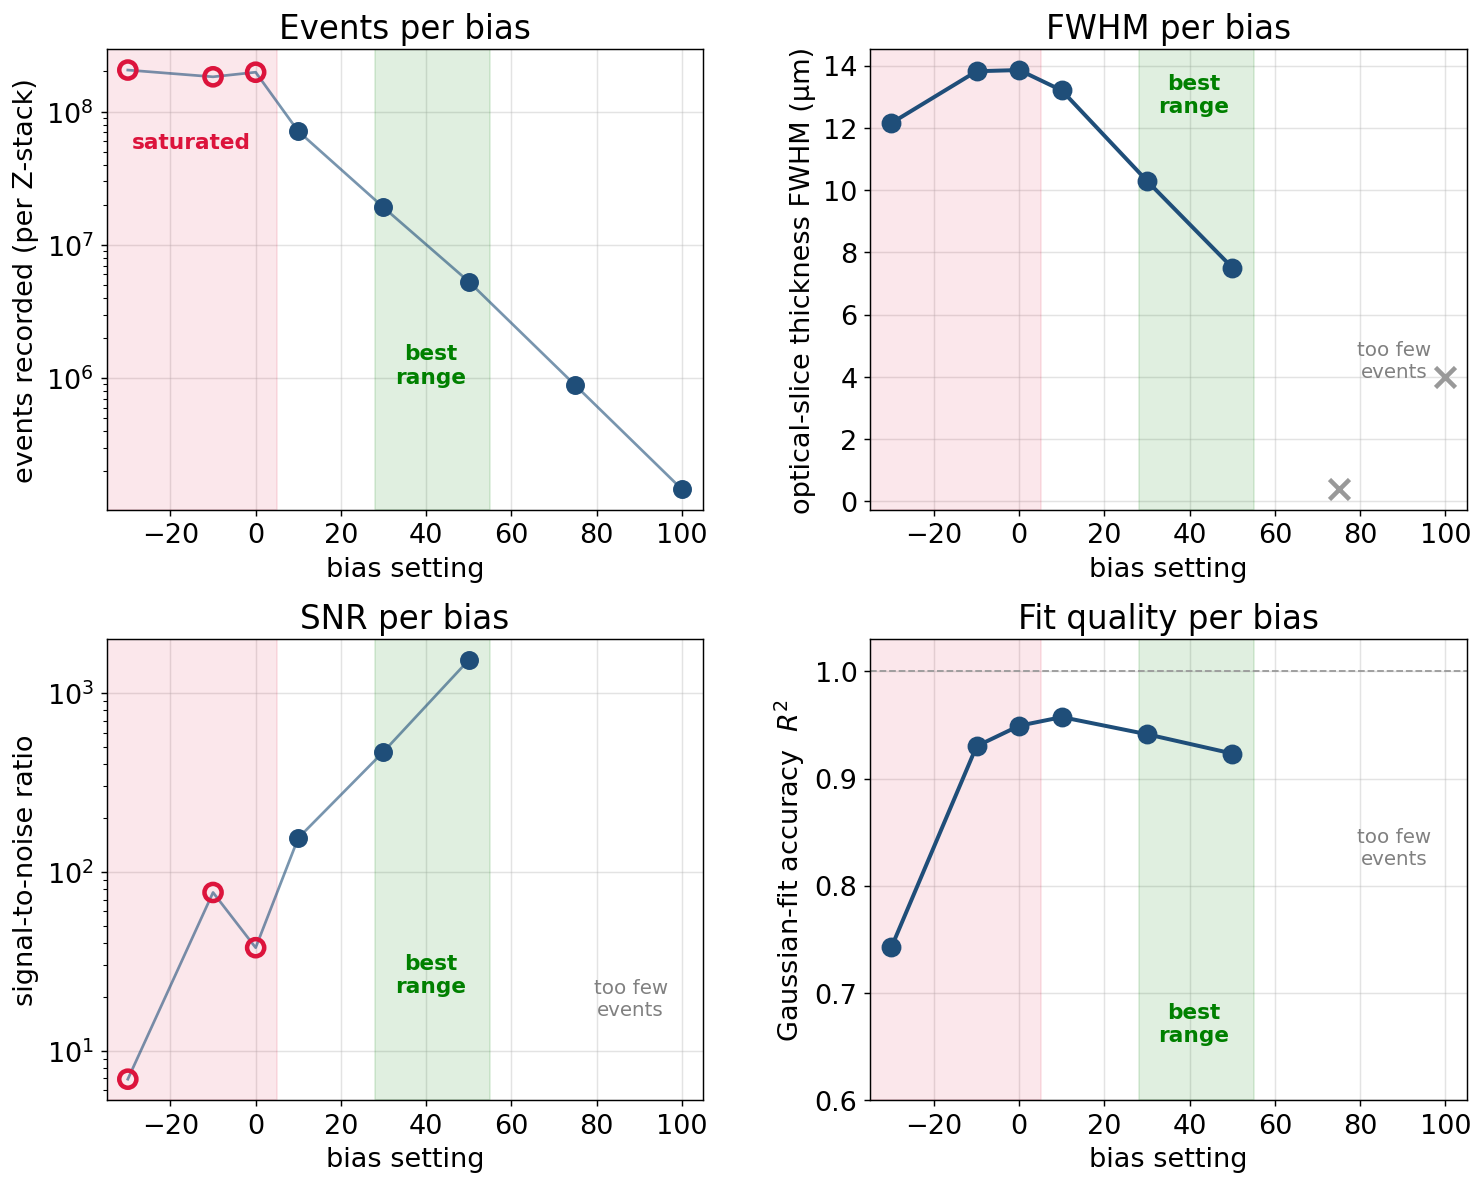
\includegraphics[width=\textwidth]{SIMPLE_overview.png}
  \caption{Summary of the bias sweep. \textbf{(top-left)} number of recorded events;
  \textbf{(top-right)} optical-slice thickness (FWHM); \textbf{(bottom-left)}
  signal-to-noise ratio; \textbf{(bottom-right)} accuracy of the Gaussian fit ($R^2$).
  Red band $=$ saturated/unusable settings; green band $=$ recommended ``best range''.}
  \label{fig:overview}
\end{figure}

%--------------------------------------------------------------------
\section{How to read the figure}

\paragraph{(a) Events per bias --- the bias is a sensitivity dial.}
The number of events drops almost perfectly exponentially: roughly \textbf{$\div 10$ for
every $+34$ bias units}. Physically, an event fires when the brightness at a pixel changes
by more than a threshold, and the bias sets that threshold. A higher bias demands a bigger
brightness change, so it produces fewer but more meaningful events. The three open red
points are saturated (Section~\ref{sec:sat}) and do not follow the line.

\paragraph{(b) FWHM per bias --- the bias sets the optical-slice thickness.}
Raising the bias removes weak out-of-focus light and keeps only the sharp in-focus speckle,
so the optical section gets \emph{thinner} (better): from $\sim$14\,$\mu$m at low bias down
to $\sim$7.5\,$\mu$m at bias~50. Beyond bias~$\sim$75 there are too few events to fit
(grey crosses).

\paragraph{(c) SNR per bias --- higher bias gives cleaner sectioning.}
The signal-to-noise ratio of the axial profile rises strongly with bias (note the log
scale), because the out-of-focus background is suppressed. It is defined as
\[
\mathrm{SNR}=\frac{I_\text{peak}-I_\text{background}}{\sigma_\text{background}},
\]
i.e.\ how far the in-focus peak rises above the out-of-focus planes, divided by their
scatter.

\paragraph{(d) Fit quality per bias --- how well the data match a Gaussian.}
This is the accuracy of the Gaussian fit used to measure the FWHM, given by the coefficient
of determination
\[
R^2 = 1-\frac{\sum_i \big(y_i-\text{model}(z_i)\big)^2}{\sum_i \big(y_i-\bar{y}\big)^2},
\]
which is the fraction of the profile's variation explained by the fit ($R^2=1$ is perfect).
In the usable range $R^2\approx 0.93$--$0.96$: the profiles are well described by a Gaussian,
but not perfectly. The small gap from~1 is consistent with the slightly tilted beam
distorting the profile. At saturation the fit degrades ($R^2=0.74$ at bias~$-30$).

%--------------------------------------------------------------------
\section{The two limits}\label{sec:sat}

\paragraph{Too low (bias $\lesssim 5$, red band): saturation.}
The camera becomes so sensitive that it produces events faster than they can be recorded.
The event rate hits a hard ceiling ($\sim$20\,Mevents/s controller cap, $\sim$9\,Mevents/s
sustained by the data link) and only about \textbf{half} of the requested recording time is
actually stored; the image floods with background events. The large event count here is an
artefact, not real signal --- like a microphone clipping. These settings are unusable.

\paragraph{Too high (bias $\gtrsim 75$): starvation.}
The threshold is so high that almost no events are produced, the signal is lost in noise,
and the Gaussian fit fails.

%--------------------------------------------------------------------
\section{Why the ``best range'' is best}
The green band (bias~$30$--$50$) is the sweet spot between the two limits. Going up from
saturation, the section gets thinner (b) and the SNR rises (c) as background is rejected ---
but this only continues until the signal itself becomes too weak (the ``too few events''
region). Bias~$30$--$50$ is where all of the following hold at once: clear of saturation,
thinnest/cleanest optical section, highest SNR, and still enough events with a good fit.

%--------------------------------------------------------------------
\section{Effect of the acquisition time (duration)}
We also varied the recording time per plane from $0.1$ to $10$\,s
(Fig.~\ref{fig:duration}). This test was done at bias~$\approx 0$, i.e.\ in the saturated
regime, and shows two effects.

\begin{itemize}
  \item \textbf{Only about half of the requested time is actually recorded}
  (Fig.~\ref{fig:duration}a). Because the camera is saturated, the data link cannot keep up,
  and the trailing events are dropped: ask for $10$\,s and you store $\sim$5\,s, ask for
  $2$\,s and you store $\sim$1\,s, and so on ($\sim$50\% at every duration).
  \item \textbf{Longer recording does not improve the sectioning}
  (Fig.~\ref{fig:duration}b): the SNR stays roughly flat ($\sim$40--80) as the time
  increases. The total number of events does grow linearly with time (the rate is pinned at
  the saturation ceiling), but those extra events are background, so the image quality does
  not improve.
\end{itemize}

\medskip
\noindent\textbf{Interpretation.}
At a saturating bias, integration time cannot fix the problem --- the limit is the
background flood, not a lack of signal. Acquisition time should therefore be chosen at a
non-saturating bias (the recommended range below), where a longer recording \emph{would}
genuinely add signal. For the recommended settings, $\sim$1\,s per plane is enough and is
fully recorded.

\begin{figure}[h]
  \centering
  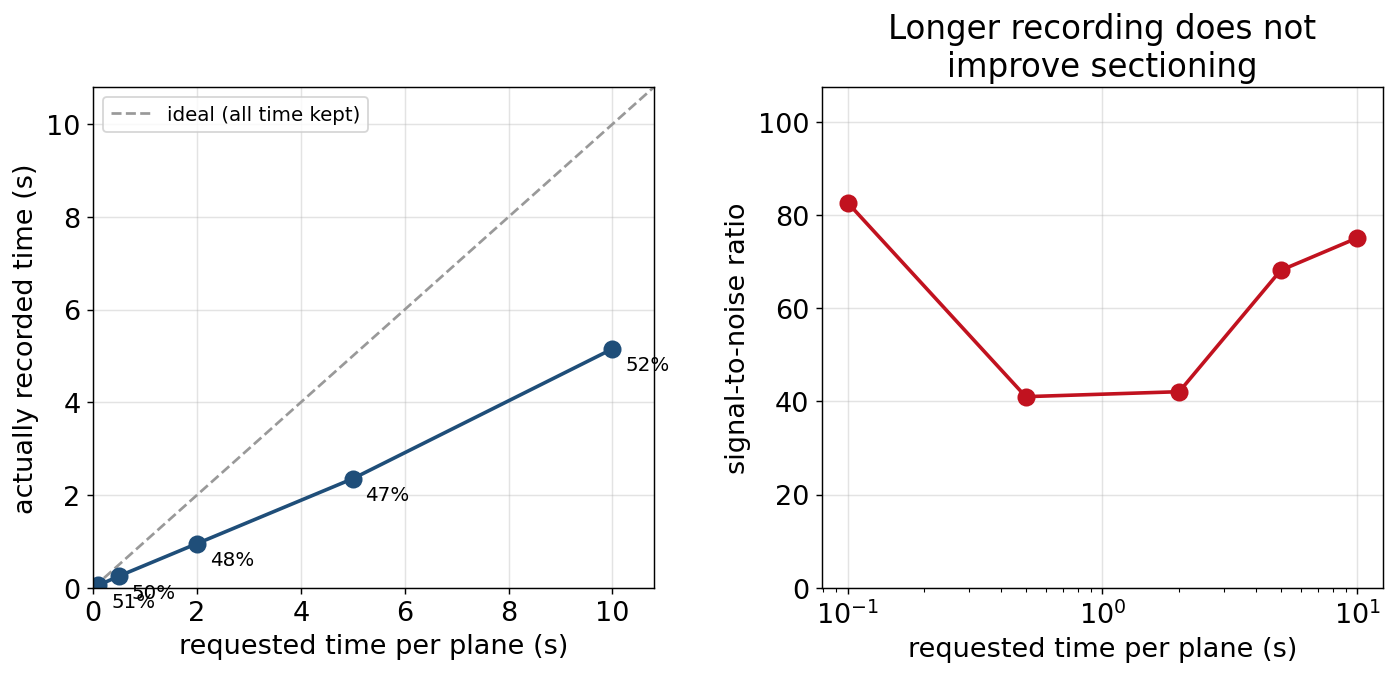
\includegraphics[width=\textwidth]{SIMPLE_duration.png}
  \caption{Effect of acquisition time (at the saturating bias~$\approx 0$).
  \textbf{(left)} only $\sim$50\% of the requested time is actually stored;
  \textbf{(right)} the sectioning SNR does not improve with longer recordings.}
  \label{fig:duration}
\end{figure}

%--------------------------------------------------------------------
\section{Summary and recommendation}

\begin{table}[h]
  \centering
  \begin{tabular}{lll}
    \toprule
    Quantity & Value & Meaning \\
    \midrule
    Events vs.\ bias       & $\div 10$ per $34$ units & bias $=$ contrast-threshold dial \\
    Event-rate ceiling     & $\sim 9$--$20$\,Mev/s    & saturation limit at low bias \\
    Captured time (saturated) & $\sim 50\%$ of request & low bias loses half the recording \\
    Section FWHM (bias $0\!\to\!50$) & $13.9 \to 7.5$\,$\mu$m & thinner $=$ better sectioning \\
    SNR (bias $0\!\to\!50$) & $\sim 40 \to 1500$       & background rejection improves \\
    Fit accuracy $R^2$     & $0.93$--$0.96$           & good Gaussian fit (mild tilt) \\
    Duration (at bias~$0$) & SNR flat $0.1\!\to\!10$\,s & time can't fix saturation \\
    \bottomrule
  \end{tabular}
  \caption{Key measured numbers.}
\end{table}

\noindent\textbf{Recommended operating point:}
\[
\boxed{\;\texttt{bias\_diff\_on} = \texttt{bias\_diff\_off} \approx 30\text{--}50,\quad
\text{full sensor},\ \sim 1\,\text{s per plane}.\;}
\]
This sits safely below saturation, gives the thinnest and cleanest optical section, and
keeps the event rate well within the data link so the full acquisition time is recorded.
Use a lower bias (10--20) only when more raw signal is needed and a thicker section is
acceptable.

\end{document}
